\xchapter{Planejamento do estudo experimental}
{...}
\label{planejamento}

Os estudos apresentados no Capítulo \ref{fundamentacao} mostram carência de estudos
sobre qualidade interna de ferramentas de análise estática, especialmente
sobre aspectos relacionados à manutenabilidade de tais ferramentas, assim
propomos neste trabalho investigar a seguinte questão de pesquisa.

\section{Questão de pesquisa}

\begin{enumerate}
  \item [{\bf Q1:}] {\em As características das ferramentas de análise estática
  de código-fonte tem impacto em sua manutenabilidade?}
\end{enumerate}

\section{Objetivo geral}

O nosso objetivo principal é compreender as ferramentas de software
para análise estática de código-fonte do ponto de vista de sua
manutenabilidade, a partir da observação de suas características e dos valores
de métricas de código-fonte. Este objetivo será alcançado através dos
seguintes objetivos específicos:

\section{Objetivos específicos}

\begin{itemize}
  \item Caracterizar as ferramentas de análise estática.
  \item Medir a manutenabilidade das ferramentas de análise estática.
  \item Compreender a relação entre características e manutenabilidade
        das ferramentas de análise estática.
\end{itemize}

A compreensão que se busca neste estudo será conduzida através de uma avaliação
empírica das características das ferramentas de análise estática e de seu nível
de manutenabilidade, este nível de manutenabilidade será dado pela
interpretação das métricas de código-fonte calculadas para este estudo. Em
consequência temos as seguintes hipóteses para testar a relação entre
características de manutenabilidade.

\section{Hipóteses} \label{hipoteses}

\begin{enumerate}
  \item[{\bf H0}] {\em Não existe correlação entre características das
  ferramentas de análise estática e sua manutenabilidade.}
  \item[{\bf H1}] {\em Existe correlação entre características das ferramentas
  de análise estática e sua manutenabilidade.}
\end{enumerate}

\section{Variáveis}

As variáveis deste estudo serão as características das ferramentas de análise
estática, como nossa variável independente, e o nível de manutenabilidade das
ferramentas de análise estática, como variável dependente.

\section{Design}

As características das ferramentas, descritas no Capítulo \ref{caracterizacao-ferramentas},
serão utilizadas para criar grupos distintos de ferramentas, estes grupos de ferramentas
serão comparados entre sí com objetivo de identificar empiricamente se as características
afetam na manutenabilidade das ferramentas.

O nível de manutenabilidade das ferramentas será dado pela interpretação das métricas de
código-fonte de complexidade estrutural e custo de mudança, para evitar influência de fatores
conhecidos nos valores destas métricas, iremos isolar estes fatores realizando comparações
entre ferramentas com os mesmos fatores, por exemplo, comparação entre linguagens diferentes,
domínio de aplicação diferentes, tamanho em número de classes.

O estudo é um experimento com um fator e mais de dois tratamentos, o fator
neste estudo é a manutenabilidade das ferramentas de análise estática e o
tratamento será uma série de comparações entre grupos distintos de ferramentas
com características comuns.

%Para garantir o princípio de ``randomization'' irei comparar com o maior número
%de características das ferramentas possíveis.
%Para garantir o princípio de ``balancing'' selecionei o mesmo número de
%releases das ferramentas que serão analisadas longitudemente.

\section{Objects}

Os objetos deste estudo serão ferramentas de análise estática de código-fonte,
sendo mais específico, iremos estudar algumas características externas destas
ferramentas bem como características internas obtidas a partir de métricas de
código-fonte, então todas as ferramentas incluídas neste estudo são ferramentas
com disponibilidade de código-fonte.

\section{Instrumentation}

A investigação será realizada a partir de uma busca e seleção de ferramentas de
análise estática, em seguida para cada ferramenta selecionada iremos obter
o código-fonte da ferramenta, com código-fonte em mão iremos calcular métricas
de complexidade estrutural e custo de mudança, em paralelo as características
dessas ferramentas serão documentadas, neste ponto a análise e interpretação
dos dados se iniciará, o objetivo será compreender quais características
implicam na manutenabilidade.

\section{Data collection procedure}

Os dados serão coletados através de uma revisão estruturada, análise estática
com o Analizo, e caracterizacao manual das ferramentas a partir das fontes:
artigo, documentação, sites e repositórios da ferramenta.

Além da revisão estruturada, que será a fonte de ferramentas da academia,
iremos também buscar e selecionar ferramentas da indústria, para isto
buscaremos fontes e catálogos através de pesquisa livre na internet.

\subsection{Revisão estruturada}

A revisão estruturada é um processo disciplinado para seleção de artigos com
publicação de ferramentas de software a partir de critérios bem definidos, de
forma que seja possível a reprodução do estudo por parte de pesquisadores
interessados. O resultado final produzido pela revisão estruturada é um conjunto
de ferramentas de software com disponibilidade de código-fonte, estas ferramentas
são disponibilizadas pelos autores dos artigos.

A revisão estruturada difere da revisão e do mapeamento sistemático
por ser um processo mais simples e menos rígido, onde o resultado final é
um conjunto de ferramentas de software, enquanto no mapeamento ou na revisão
sistemática há um esforço em caracterizar os artigos analisados o mesmo
não ocorre na revisão estruturada.

A revisão estruturada é organizada em três atividades de (1) busca de artigos
(definição das fontes, obtenção dos artigos nas fontes), (2) filtro (definição
de critérios de busca, definição de script de busca) e (3) seleção de artigos
com publicação de ferramentas conforme representado na Figura
\ref{figura-revisao-estruturada}.

\begin{figure}[h]
  \center
  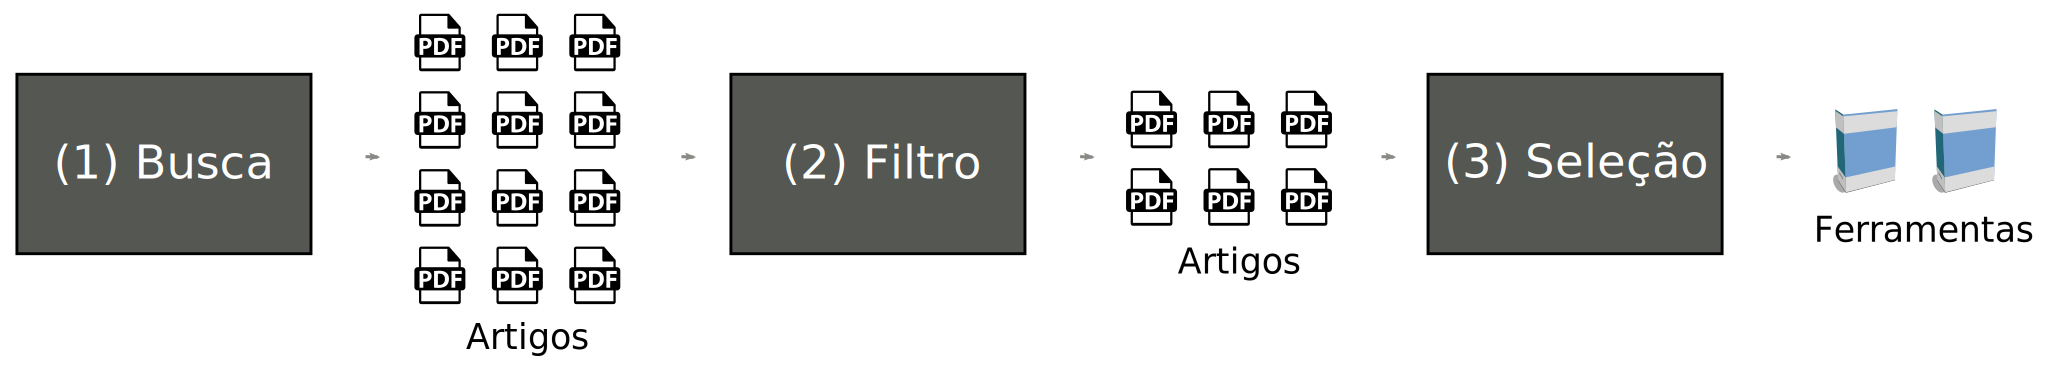
\includegraphics[scale=0.33]{imagens/revisao-estruturada.png}
  \caption{Representação gráfica da revisão estruturada}
  \label{figura-revisao-estruturada}
\end{figure}

Na primeira atividade da revisão estruturada são definidas as fontes de busca,
estas fontes são conferências que abordam o tema de interesse do estudo, e que
apresentem um grande potencial de encontrarmos ferramentas de análise estática
de código-fonte publicadas em suas inúmeras edições.

Esta primeira atividade de busca passa então pelo maior número de ediçoes das
conferências, e para cada edição são copiados localmente os
artigos em seu formato PDF para posterior filtro na etapa seguinte,

A segunda atividade da revisão estruturada realizada em cima deste conjunto inicial
é um filtro realizado de forma automática com o auxílio do script
{\it
filter}\footnote{http://github.com/joenio/dissertacao-ufba-2016/blob/master/revisao-estruturada/filter}
escrito especialmente para este estudo. Este script busca em todo o conteúdo
dos artigos os seguintes termos:

\begin{verbatim}
  "tool" OU "framework"; E
  "download" OU "available"; E
  "http" OU "ftp"; E
  "static analysis" OU "parser".
\end{verbatim}

A terceira e última atividade da revisão estruturada,
seleção de artigos, pretende identificar se cada artigo
resulta, de fato, em publicação de ferramenta de análise estática. Esta seleção
é feita a partir de uma leitura superficial do artigo em busca de indícios de
que o artigo publica uma ferramenta. Ferramentas que sejam mais abrangentes do
que apenas análise estática mas que contenham esta função em seu conjunto
também serão selecionadas.

Artigos que citam que desenvolveram alguma ferramenta, protótipo ou prova de
conceito mas não dão nenhum detalhes sobre a ferramenta, como nome ao menos,
não serão incluídos na caracterização das ferramentas.

Uma vez identificados os artigos que publicaram ferramentas de análise
estática, procuramos no próprio artigo por referências de onde encontrar o
código-fonte da ferramenta. Neste contexto, algumas ações serão tomadas a
partir de algumas situações.

\begin{itemize}

  \item Se os autores afirmam que a ferramenta está disponível mas o artigo
    não contém referências de onde encontrar o código-fonte, então estes
    autores serão contactados, por email, solicitando informações de onde
    obter o código-fonte da ferramenta.

  \item Se o artigo indica onde obter o código-fonte da ferramenta, mas o acesso ao local
    indicado não está disponível, ou está disponível mas o software não se
    encontra lá, então os autores serão contactados, solicitando informações
    atualizadas de onde obter uma cópia do código-fonte da ferramenta.

  \item Artigos que indicam onde obter o código-fonte da ferramenta e a referência
    está correta. Será feito o download do código-fonte da última versão
    disponível.

\end{itemize}

Uma vez que os autores contactados por email respondam com informações sobre
local para obter o software, iremos adicionar a ferramenta ao conjunto de ferramentas
a serem analisadas.

O código-fonte da versão mais recente de cada uma destas ferramentas foi
copiado localmente para caracterização e análise através da coleta de suas
métricas de código-fonte.
'
\subsection{Ferramentas da indústria}

Em paralelo à revisão estruturada para seleção de ferramentas da academia
será realizada uma seleção manual não estruturada para busca de ferramentas da indústria.

Esta busca se justifica pois a caracterização das ferramentas da academia será feita lado a
lado às ferramentas da indústria a fim de traçar paralelo entre estes dois contextos, onde
poderemos verificar se existem diferenças entre as características destes dois mundos e
se for o caso explicar tais diferenças.

As ferramentas selecionadas para o estudo serão analisadas terão suas métricas
calculadas, bem como serão caracterizadas a partir de algumas dimensões para
posterior análise.

\subsection{Caracterização das ferramentas de análise estática}

As ferramentas de análise estática selecionadas serão caracterizadas
a partir de algumas dimensões que se mostrem necessárias ao nosso estudo, todas
as ferramentas foram obtidas em sua versão mais recente, apenas uma única versão
de cada ferramenta foi selecionada e será caracterizada a partir de tal versão,
esta cópia de cada ferramenta foi do seu código-fonte, algumas características
são obtidas do código-fonte, outras da documentação da ferramenta.

Esta caracterização será fundamental para compreender as métricas de código-fonte
extraídas destas ferramentas,
ferramentas que tenham interface gráfica de usuário por exemplo podem apresentar
valores diferentes daquelas que tenham apenas interface modo texto, suporte
a analisar múltiplas linguagens pode também trazer valores de métricas maiores ou
piores. Iremos levar estas características em consideração durante a análise
exploratória dos nosso dados.

Para compor as características e também evitar re-criar dimensões para características
de ferramentas deste domínio iremos nos basear no trabalho de
\citeonline{Novak2010}, onde um estudo para construção de uma taxonomia para
ferramentas de análise estática propuseram uma classificação a partir de uma
série de categorias.

Iremos utilizar algumas de suas características, apenas aquelas que nos forem necessárias
para interpretar e caracterizar a complexidade estrutural de tais ferramentas, segue abaixo todas
as características proposta no trabalho de \citeonline{Novak2010}.

\begin{description}

  \item {\it Entrada - quais tipos de arquivos podem ser carregados na ferramenta:}
    \begin{itemize}
      \item Código-fonte - arquivos de código texto podem ser carregados
      \item Byte code - arquivos com Java Byte Code ou Microsoft
      \item Linguagem intermediária (MSIL) pode ser carregada
    \end{itemize}

  \item {\it Lançamentos ({\it Releases}) - quantos lançamentos por ano:}
    \begin{itemize}
      \item Frequentemente $>=$ 3 vezes ao ano - novas versões da ferramenta são lançadas 3 ou mais vezes por ano
      \item Ocasionalmente $<$ 3 vezes ao ano - novas versões da ferramenta são lançadas menos que 3 vezes ao ano
      \item Obsoleta 0 vezes ao ano - intervalo entre novos lançamentos é maior que 1 ano
    \end{itemize}

  \item {\it Linguagens suportadas - quais linguagens de programação a ferramenta suporta:}
    \begin{itemize}
      \item .NET - todas as linguagens compiladas em bibliotecas ou programas no framework .NET
      \item VB .NET - suporta VB.NET
      \item C\# - suporta C\#
      \item Java - suporta linguagem de programação Java
      \item C, C++ - suporta linguagem de programação C ou C++
    \end{itemize}

  \item {\it Tecnologia - quais tecnologias são usadas para procurar erros no código:}
    \begin{itemize}
      \item Dataflow - busca por erros com dataflow
      \item Sintaxe - busca por errors de sintaxe e correctness
      \item Prova de teoremas - procurar erros em provar diferentes teoremas
      \item Verificação de modelos - procurar erros com verificação de modelo
    \end{itemize}

  \item {\it Regras - conjunto de regras, quais são suportadas por diferentes código estático:}
    \begin{itemize}
      \item Estilo - inspeciona a aparência do código-fonte
      \item Naming - checa se as varáveis são nomeadas corretamente (ortografia, padroes de nomenclatura, ...)
      \item Geral - regras gerais de analise estática de código
      \item Concorrencia - erros com execução de código de concorrente
      \item Exceções - erros lançando ou não exceções
      \item Performance - erros de performance das aplicações
      \item Interoperabilidade - erros de comportamento comum
      \item Segurança - erros que podem impactar na segurança da aplicação
      \item SQL - procurar por "SQL injections" e outros erros de SQL
      \item Buffer overflow - erros de segurança, que explorar buffer overflow
      \item Manutenabilidade - regras para melhor manutenabilidade da aplicação
    \end{itemize}

  \item {\it Configurabilidade - habilidade de configurar a ferramenta:}
    \begin{itemize}
      \item Documento texto - comfiguração é feita via documento texto
      \item XML - configuração pe feita por documento XML
      \item GUI - configuraçãi é feita via interface gráfica
      \item Ruleset - ferramenta pode ligar/desligar conjunto de regras
    \end{itemize}

  \item {\it Extensibilidade - se a ferramenta pode ser extendida com regras próprias:}
    \begin{itemize}
      \item Possível - é possível extender
      \item Não possível - não é possível extender
    \end{itemize}

  \item {\it Disponibilidade - de que forma a ferramenta está disponível:}
    \begin{itemize}
      \item Código Aberto ({\it Open Source}) - a ferrament é livre e o código-fonte está disponível
      \item Grátis ({\it Free}) - a ferramenta é grátis mas o código-fonte não está disponível
      \item Comercial - a ferramenta está disponível mediante pagamento
    \end{itemize}

  \item {\it Experiência do usuário - de que forma a ferramenta pode ser usada, como é oferecida:}
    \begin{itemize}
      \item Integração com ambiente - como a ferramenta é integrada ao ambiente de trabalho
      \item Localização automática de erros no código - quando a ferramenta encontra um erro, ela leva ao local do erro
      \item Ajuda abrangente sobre falhas - se a ferramenta oferece ajuda na resolução de erros
      \item Interface de usuário - disponibilidade de uma interface de usuário
      \item Linha de comando - ela pode ser executada via linha de comando
      \item GUI - a ferramente pode ser executada em uma interface gráfica (GUI)
    \end{itemize}

  \item {\it Saída - representação dos resultados da ferramenta:}
    \begin{itemize}
      \item Arquivo texto - ferramenta pode apresentar resultados em arquivos texto
      \item Lista - ferramenta pode apresentar resultados numa interface de usuário customizada controlada em GUI
      \item Arquivo XML - ferramenta pode apresentar resultados em dados XML
      \item Arquivo HTML - ferramenta pode apresentar resultados em dados HTML
    \end{itemize}

\end{description}

Iremos utilizar algumas destas categorias na caracterização das ferramentas
selecionadas neste estudo, e vamos também caracterizar em relação à algumas dimensões que nos
foram necessárias mas que não faziam parte das dimensões propostas por \citeonline{Novak2010},
estas dimensões são as seguintes.

\begin{description}

  \item {\it Linguagem de programação - em que linguagem de programação à ferramenta é escrita:}
    \begin{itemize}
      \item .NET
      \item VB .NET
      \item C\#
      \item Java
      \item C, C++
    \end{itemize}

  \item {\it Tamanho em número de classes - número de classes/módulos da ferramenta}

  \item {\it Contexto - onde a ferramenta surgiu:}
    \begin{itemize}
      \item Academia
      \item Indústria
    \end{itemize}

\end{description}


\section{Analysis procedure}

\section{Evaluation of validity}
